\documentclass[12pt]{article}
\usepackage[margin=1in]{geometry}
\usepackage{graphicx}
\usepackage{listings}
\usepackage{xcolor}
\usepackage{amsmath}
\usepackage{booktabs}
\usepackage{hyperref}
\usepackage{caption}
\usepackage{float}
\usepackage{amssymb}
\usepackage{textcomp}
\usepackage{titlesec}
\usepackage{parskip}

% Code listing style
\lstdefinestyle{ros}{
    backgroundcolor=\color{gray!10},
    basicstyle=\ttfamily\small,
    keywordstyle=\color{blue},
    commentstyle=\color{green!50!black},
    stringstyle=\color{red!70!black},
    breaklines=true,
    frame=single,
    numbers=left,
    numberstyle=\tiny\color{gray},
    tabsize=4,
    showstringspaces=false
}

\lstdefinestyle{bash}{
    backgroundcolor=\color{black!90},
    basicstyle=\ttfamily\small\color{white},
    breaklines=true,
    frame=single,
    showstringspaces=false
}

\title{
    \vspace{-1cm}
    \large RBE 500 --- Foundations of Robotics \\[0.4em]
    \LARGE \textbf{Project Assignment 2} \\[0.4em]
    \large Worcester Polytechnic Institute
}
\author{Tracy Yang \and Kyle Yee}
\date{\today}

\begin{document}

\maketitle

% ===========================================================================
\section{Fix the Joints}
% ===========================================================================

\subsection{Overview}

For this assignment, joints 1 and 2 were fixed so that only the last joint
(joint 3, the prismatic joint) remains active. This was done by changing the
\texttt{type} attribute of \texttt{joint\_1} and \texttt{joint\_2} from
\texttt{revolute} to \texttt{fixed} in the URDF.

\subsection{URDF Frame Correction}

The PA1 feedback noted that the URDF and FK frames did not match. The root
cause was that \texttt{joint\_1}'s origin was placed at the bottom of the
column (\texttt{z=0.05}), while the DH convention places Frame~1 at the
shoulder (top of the column). This split the $d_1$ offset across two joints
(\texttt{joint\_1} and the fixed \texttt{arm\_1\_attach}), causing a mismatch.

The fix was to move \texttt{joint\_1}'s origin to \texttt{z=0.5}
($= 0.05_{\text{base}} + 0.45_{\text{column}}$), placing Frame~1 directly at
the shoulder where $a_1$ begins. The \texttt{link\_1} visual origin was adjusted
to \texttt{z=-0.225} so the column geometry remains in the correct world
position. The DH parameters now match the URDF exactly:

\begin{table}[H]
\centering
\caption{SCARA DH Parameters (corrected)}
\label{tab:dh}
\begin{tabular}{lll}
\toprule
\textbf{Parameter} & \textbf{Symbol} & \textbf{Value} \\
\midrule
Joint 1 $z$-offset (base to shoulder) & $d_1$ & 0.50 m \\
Arm 1 length                           & $a_1$ & 0.40 m \\
Link 2 length                          & $a_2$ & 0.30 m \\
Joint 3 range                          & $d_3$ & $[-0.2,\, 0.2]$ m \\
\bottomrule
\end{tabular}
\end{table}

\begin{lstlisting}[style=ros, language=XML,
    caption={Fixed URDF joints. Joint 1 origin corrected to z=0.5;
             joints 1 and 2 set to fixed type.}]
<!-- joint_1: FIXED, origin raised to z=0.5 to match DH Frame 1 -->
<joint name="joint_1" type="fixed">
    <parent link="base_link"/><child link="link_1"/>
    <origin xyz="0 0 0.5"/>
    <axis xyz="0 0 1"/>
</joint>

<!-- arm_1_attach: origin collapsed to 0 (offset now in joint_1) -->
<joint name="arm_1_attach" type="fixed">
    <parent link="link_1"/><child link="arm_1"/>
    <origin xyz="0 0 0"/>
</joint>

<!-- joint_2: FIXED -->
<joint name="joint_2" type="fixed">
    <parent link="arm_1"/><child link="link_2"/>
    <origin xyz="0.4 0 0"/>
    <axis xyz="0 0 1"/>
</joint>

<!-- joint_3: ACTIVE (prismatic, last joint) -->
<joint name="joint_3" type="prismatic">
    <parent link="link_2"/><child link="link_3"/>
    <origin xyz="0.3 0 0"/>
    <axis xyz="0 0 1"/>
    <limit effort="1000" lower="-0.2" upper="0.2" velocity="0.5"/>
</joint>
\end{lstlisting}

% ===========================================================================
\section{Position Controller Node}
% ===========================================================================

\subsection{Architecture Overview}

The controller was implemented as a new ROS2 Python package
(\texttt{scara\_controller}). The overall architecture is:

\begin{itemize}
    \item \textbf{Subscriber}: \texttt{/joint\_states}
          (\texttt{sensor\_msgs/JointState}) --- reads joint\_3 position
          from Gazebo via the \texttt{ros\_gz\_bridge}.
    \item \textbf{Publisher}: \texttt{/scara/joint3\_cmd}
          (\texttt{std\_msgs/Float64}) --- publishes the computed PD effort
          to Gazebo via bridge.
    \item \textbf{Service}: \texttt{/scara/set\_joint3\_position}
          (\texttt{scara\_ik/SetJointPosition}) --- accepts a reference
          position and stores it as the controller setpoint.
    \item \textbf{Control loop}: 100~Hz timer executing the PD law.
\end{itemize}

The effort value is delivered to Gazebo through the
\texttt{gz-sim-joint-position-controller-system} plugin with gains set to
$p=1$, $i=0$, $d=0$, making it act as a direct pass-through. This ensures
the force computed by the ROS2 node is applied exactly as-is inside the
Gazebo physics loop, which resolves the WSL2 clock desynchronization that
prevented reliable force application via \texttt{apply\_joint\_effort}.

\subsection{Reading Joint States (Part 2a)}

The node subscribes to \texttt{/joint\_states}, which is bridged from the
Gazebo joint state publisher plugin. The joint\_3 position is extracted by
name lookup:

\begin{lstlisting}[style=ros, language=Python,
    caption={Joint state subscriber callback}]
def joint_state_cb(self, msg: JointState):
    """Read joint_3 position from the Gazebo-bridged joint state."""
    if 'joint_3' in msg.name:
        idx = msg.name.index('joint_3')
        self.cur_position = msg.position[idx]
\end{lstlisting}

The Gazebo joint state publisher plugin (in \texttt{scara.urdf}) publishes
only \texttt{joint\_3} since joints 1 and 2 are fixed:

\begin{lstlisting}[style=ros, language=XML,
    caption={Gazebo joint state publisher plugin (URDF)}]
<gazebo>
    <plugin filename="gz-sim-joint-state-publisher-system"
            name="gz::sim::systems::JointStatePublisher">
        <topic>/world/empty/model/scara/joint_state</topic>
        <joint_name>joint_3</joint_name>
    </plugin>

    <plugin filename="gz-sim-joint-position-controller-system"
            name="gz::sim::systems::JointPositionController">
        <joint_name>joint_3</joint_name>
        <topic>/scara/joint3_cmd</topic>
        <p_gain>1</p_gain>
        <i_gain>0</i_gain>
        <d_gain>0</d_gain>
    </plugin>
</gazebo>
\end{lstlisting}

\subsection{PD Controller Design (Part 2b)}

A PD controller was designed for joint\_3. Since no analytical model was
required, the gains were tuned empirically. The control law is:

\[
u(t) = K_p \, e(t) + K_d \, \dot{e}(t)
\]

where $e(t) = q_{\text{ref}} - q_{\text{cur}}$ is the position error and
$\dot{e}(t)$ is approximated by a finite difference at each timestep:

\[
\dot{e}(t) \approx \frac{e(t) - e(t - \Delta t)}{\Delta t}
\]

The tuned gains are $K_p = 800$ N/m and $K_d = 80$ N$\cdot$s/m.

\begin{lstlisting}[style=ros, language=Python,
    caption={PD control loop in \texttt{controller\_node.py}}]
def control_loop(self):
    """PD control law executed at 100 Hz."""
    now = self.get_clock().now()

    if self.prev_time is None:
        self.prev_time = now
        return

    dt = (now - self.prev_time).nanoseconds * 1e-9
    if dt <= 0.0:
        return
    self.prev_time = now

    # PD law
    error     = self.ref_position - self.cur_position
    error_dot = (error - self.prev_error) / dt
    self.prev_error = error

    effort = KP * error + KD * error_dot
    effort = max(-EFFORT_LIMIT, min(EFFORT_LIMIT, effort))

    msg = Float64()
    msg.data = effort
    self.cmd_pub.publish(msg)
\end{lstlisting}

\subsection{Reference Position Service (Part 2c)}

A custom service \texttt{scara\_ik/srv/SetJointPosition} was added to the
existing \texttt{scara\_ik} package (alongside \texttt{ScaraIK.srv}):

\begin{lstlisting}[style=ros, caption={SetJointPosition.srv}]
float64 position
---
bool success
string message
\end{lstlisting}

The service callback validates the requested position against joint limits
before updating the controller setpoint:

\begin{lstlisting}[style=ros, language=Python,
    caption={Service callback in \texttt{controller\_node.py}}]
def set_position_cb(self, request, response):
    target = request.position

    if not (J3_MIN <= target <= J3_MAX):
        response.success = False
        response.message = (
            f'Requested {target:.4f} m outside limits '
            f'[{J3_MIN}, {J3_MAX}] m.'
        )
        self.get_logger().warn(response.message)
        return response

    self.ref_position = target
    response.success = True
    response.message = f'Reference position set to {target:.4f} m'
    self.get_logger().info(response.message)
    return response
\end{lstlisting}

The service is called from the terminal as:

\begin{lstlisting}[style=bash]
ros2 service call /scara/set_joint3_position \
    scara_ik/srv/SetJointPosition "{position: -0.1}"
\end{lstlisting}
and
\begin{lstlisting}[style=bash]
ros2 service call /scara/set_joint3_position \
    scara_ik/srv/SetJointPosition "{position: 0.2}"
\end{lstlisting}

\subsection{Plotting Current and Reference Postions of Joint 3 (Part 2d)}

\subsection{Results}

\begin{figure}[H]
    \centering
    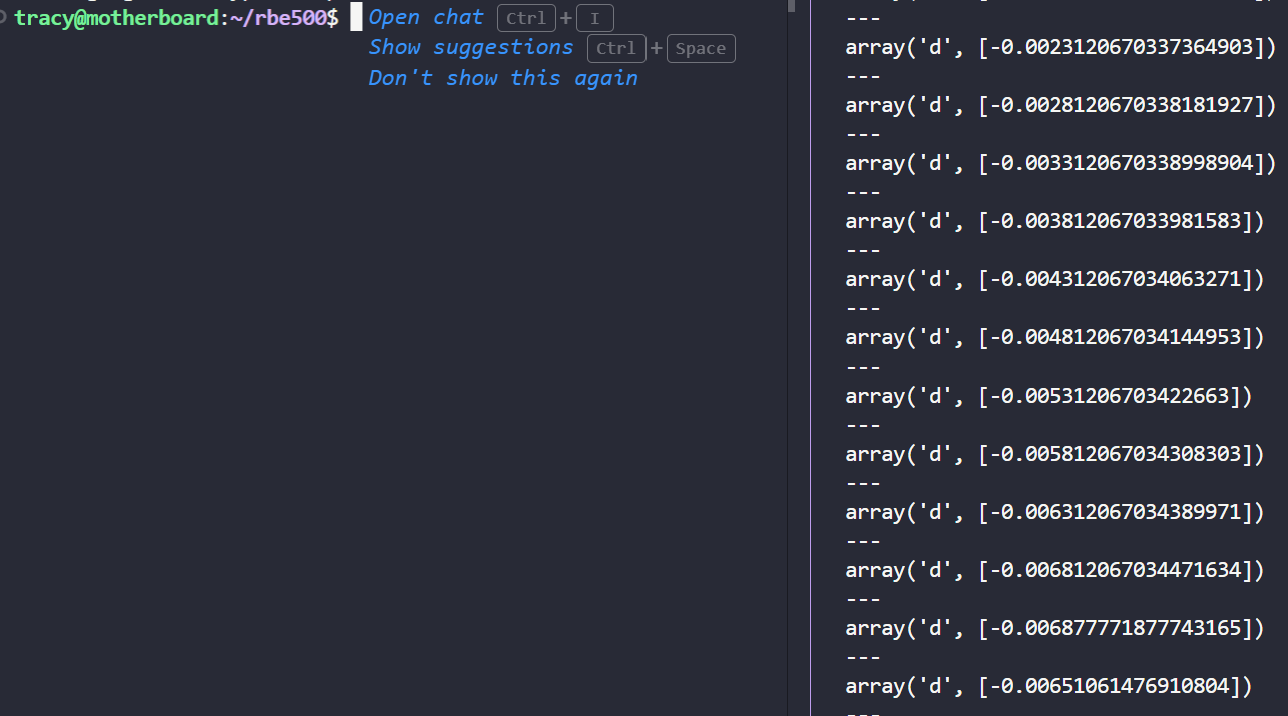
\includegraphics[width=0.85\textwidth]{screenshots/position_start.png}
    \caption*{(a) Start: $d_3 = 0.0$ m}
    \vspace{0.5em}
    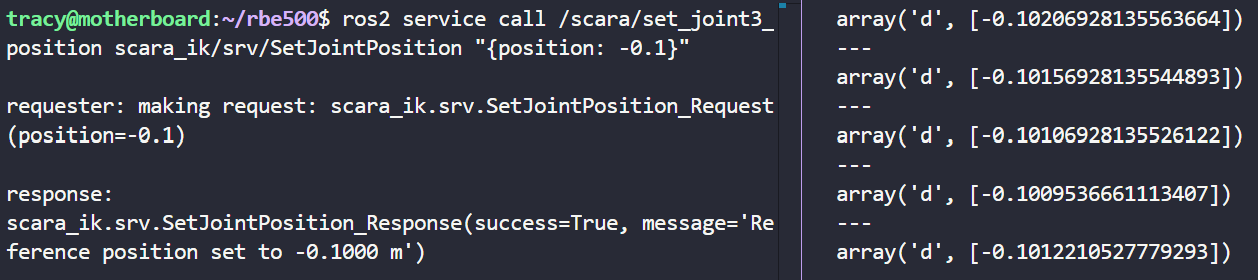
\includegraphics[width=0.85\textwidth]{screenshots/position_-0.1.png}
    \caption*{(b) Reference: $d_3 = -0.1$ m}
    \vspace{0.5em}
    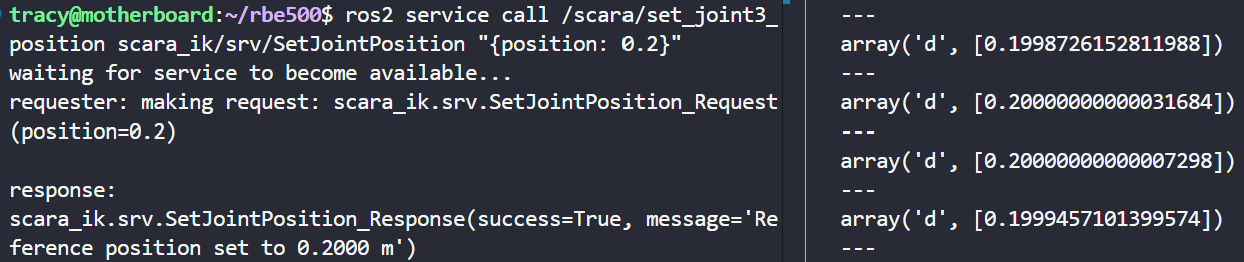
\includegraphics[width=0.85\textwidth]{screenshots/position_0.2.png}
    \caption*{(c) Reference: $d_3 = 0.2$ m}
    \caption{Joint 3 position tracking three reference commands. The PD controller
             drives the prismatic joint to each target with no steady-state error.}
    \label{fig:response}
\end{figure}

\begin{figure}[H]
    \centering
    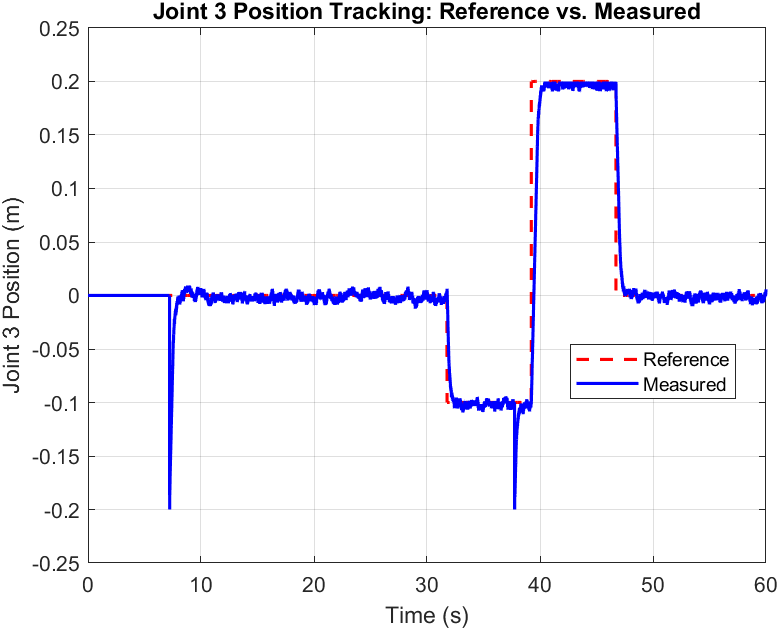
\includegraphics[width=0.85\textwidth]{screenshots/matlab_plot.png}
    \caption{MATLAB plot of reference position vs.\ measured joint\_3 position
             over time. % TODO: add after Part 2d
            }
    \label{fig:matlab}
\end{figure}

% ===========================================================================
\section{Package Structure}
% ===========================================================================

The submission adds two packages to the existing \texttt{ros2\_ws/src/}
workspace from PA1:

\begin{itemize}
    \item \texttt{scara\_description} --- updated URDF (joints fixed,
          frame corrected, Gazebo plugins added) and updated launch file
          (effort bridge, controller node).
    \item \texttt{scara\_controller} --- PD controller node
          (\texttt{controller\_node.py}, \texttt{ament\_python}).
    \item \texttt{scara\_ik} --- extended with \texttt{SetJointPosition.srv}.
\end{itemize}

\end{document}
